\chapter{Differential-Drive Theory}

\section{Why RUDRA is a differential-drive robot}

RUDRA steers by commanding different speeds on the left and right sides. If both sides move forward at the same speed, the rover translates forward. If the right side is faster than the left, the rover turns left. If the two sides move in opposite directions, the rover spins about a point near its center.

\begin{figure}[htbp]
\centering
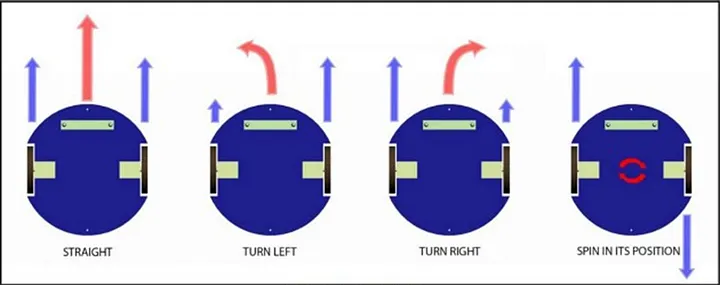
\includegraphics[width=0.72\linewidth]{figures/photos/differential_turn_modes_legacy.png}
\caption{Differential-drive motion modes: straight, turn, rotate, and spin-in-place behavior.}
\end{figure}

Although RUDRA has four wheels, the control abstraction is two-sided: a left virtual wheel and a right virtual wheel. Each virtual side represents the average ground speed of the two wheels on that side.

\section{Forward kinematics}

Let:

\begin{align*}
R &= \text{wheel radius},\\
L &= \text{distance between left and right wheel centerlines},\\
\omega_r &= \text{right wheel angular speed},\\
\omega_l &= \text{left wheel angular speed},\\
v &= \text{body forward speed},\\
\Omega &= \text{body yaw rate}.
\end{align*}

The wheel linear speeds are:

\begin{align}
v_r &= R\omega_r,\\
v_l &= R\omega_l.
\end{align}

The body forward speed and yaw rate are:

\begin{align}
v &= \frac{v_r+v_l}{2} = \frac{R}{2}(\omega_r+\omega_l), \label{eq:body-v}\\
\Omega &= \frac{v_r-v_l}{L} = \frac{R}{L}(\omega_r-\omega_l). \label{eq:body-w}
\end{align}

The planar pose is:

\begin{equation}
\mathbf{x}=\begin{bmatrix}x & y & \theta\end{bmatrix}^T.
\end{equation}

Its continuous-time derivative is:

\begin{equation}
\dot{\mathbf{x}} =
\begin{bmatrix}
\dot{x}\\ \dot{y}\\ \dot{\theta}
\end{bmatrix}
=
\begin{bmatrix}
v\cos\theta\\ v\sin\theta\\ \Omega
\end{bmatrix}.
\label{eq:pose-derivative}
\end{equation}

\section{Inverse kinematics}

ROS navigation and teleoperation commonly express a mobile-base command as \cmd{Twist}: linear velocity \(v\) and angular velocity \(\Omega\). RUDRA must convert that into side speeds:

\begin{align}
v_l &= v - \frac{\Omega L}{2}, \label{eq:left-side-speed}\\
v_r &= v + \frac{\Omega L}{2}. \label{eq:right-side-speed}
\end{align}

If wheel angular speeds are needed:

\begin{align}
\omega_l &= \frac{v_l}{R}=\frac{2v-\Omega L}{2R},\\
\omega_r &= \frac{v_r}{R}=\frac{2v+\Omega L}{2R}.
\end{align}

\begin{figure}[htbp]
\centering
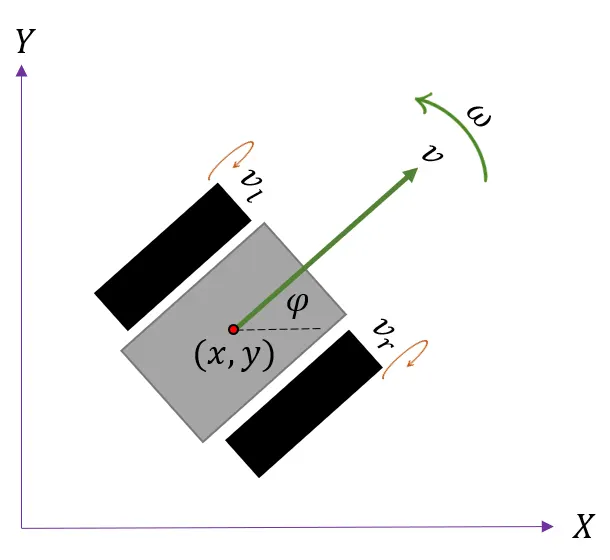
\includegraphics[width=0.55\linewidth]{figures/photos/diff_drive_frame_legacy.png}
\caption{Differential-drive coordinate frame and wheel-speed notation.}
\end{figure}

\section{Discrete odometry}

For telemetry, the Teensy can estimate wheel linear speed from encoder counts. If \(\Delta n\) counts are observed over \(\Delta t\), encoder counts per revolution are \(N\), and wheel radius is \(R\), then:

\begin{equation}
v_{wheel} = \frac{\Delta n}{N}\frac{2\pi R}{\Delta t}.
\label{eq:encoder-speed}
\end{equation}

RUDRAv4 firmware uses \(R=0.0675\) m, \(L=0.29\) m, and \(N=1683\) counts per revolution in the IMU/odometry Teensy sketch. Left and right side speeds are averaged from two encoders per side:

\begin{align}
v_l &= \frac{v_{L1}+v_{L2}}{2},\\
v_r &= \frac{v_{R1}+v_{R2}}{2}.
\end{align}

The firmware then computes:

\begin{align}
v_x &= \frac{v_l+v_r}{2},\\
\Omega_{enc} &= \frac{v_r-v_l}{L}.
\end{align}

For a sample period \(\Delta t\):

\begin{align}
\Delta \theta_{enc} &= \Omega_{enc}\Delta t,\\
\theta_k &= \theta_{k-1} + \Delta \theta,\\
x_k &= x_{k-1} + v_x\Delta t\cos(\theta_k),\\
y_k &= y_{k-1} + v_x\Delta t\sin(\theta_k).
\end{align}

The current firmware optionally blends encoder yaw increment and gyro yaw increment:

\begin{equation}
\Delta\theta = \alpha\Delta\theta_{enc} + (1-\alpha)\omega_{z,imu}\Delta t,
\end{equation}

where the present sketch uses \(\alpha=0.5\). This is a simple complementary blend in firmware; the ROS-side EKF is still the proper place to perform state estimation once the raw signals are stable.

\section{Command normalization to Sabertooth range}

The Teensy expects signed integer side commands:

\begin{equation}
u_l,u_r \in [-127,127].
\end{equation}

The \pkg{cmd_vel_to_teensy} bridge converts \topic{/cmd_vel} into side speeds and normalizes by the configured maximum linear speed:

\begin{align}
\tilde{u}_l &= \mathrm{sat}\left(\frac{v_l}{v_{max}},-1,1\right),\\
\tilde{u}_r &= \mathrm{sat}\left(\frac{v_r}{v_{max}},-1,1\right),\\
u_l &= \mathrm{round}(127\tilde{u}_l),\\
u_r &= \mathrm{round}(127\tilde{u}_r).
\end{align}

This is not closed-loop wheel-speed control. It is a bounded open-loop command mapping. The present design intentionally brings up serial, telemetry, LiDAR guard, and localization before adding wheel PID.

\section{Manual joystick mixing}

The PS2 bridge uses tank-style mixing from joystick throttle and steering:

\begin{align}
u_{throttle} &= f(\text{Ly}),\\
u_{steer} &= f(\text{Rx}),\\
u_l &= \mathrm{sat}(u_{throttle}-u_{steer}, -127, 127),\\
u_r &= \mathrm{sat}(u_{throttle}+u_{steer}, -127, 127).
\end{align}

The axis mapping function centers the raw PS2 value around 127, scales it by 127, applies a deadband, and clamps the result to the Sabertooth command range. The important practical consequence is that a noisy joystick center does not command motion.

\section{Why PID is not yet the first control problem}

A PID loop is useful only after the sensing and command chain is trustworthy. RUDRAv4 has the correct staging order:

\begin{enumerate}
  \item Verify PS2 packets and \topic{/cmd_vel} mapping.
  \item Verify Teensy drive packet acknowledgement and motor directions.
  \item Verify encoder sign, scale, and side assignment.
  \item Verify IMU scale and yaw sign.
  \item Verify odometry and TF consistency.
  \item Add PID only after the open-loop system is observable.
\end{enumerate}

A wheel PID loop would compare target wheel speed and measured wheel speed:

\begin{equation}
e(t)=v_{target}(t)-v_{measured}(t),
\end{equation}

and compute:

\begin{equation}
u(t)=K_p e(t)+K_i\int_0^t e(\tau)d\tau+K_d\frac{de(t)}{dt}.
\end{equation}

But if encoder polarity, CPR, radius, sample time, or side mapping is wrong, PID will hide or amplify the wrong problem. The current open-loop base is therefore the correct commissioning foundation.
